% Created 2022-06-03 Fri 15:24
% Intended LaTeX compiler: pdflatex
\documentclass[11pt]{article}
\usepackage[utf8]{inputenc}
\usepackage[T1]{fontenc}
\usepackage{graphicx}
\usepackage{longtable}
\usepackage{wrapfig}
\usepackage{rotating}
\usepackage[normalem]{ulem}
\usepackage{amsmath}
\usepackage{amssymb}
\usepackage{capt-of}
\usepackage{hyperref}
\usepackage{cleveref}
\usepackage{subfig}
\usepackage[letterpaper, margin=1in]{geometry}
\usepackage{fancyhdr}
\pagestyle{fancy}
\usepackage{amssymb}
\usepackage{soul}
\usepackage{color}
\usepackage[citestyle=authoryear,bibstyle=authoryear, hyperref=true,backref=true,maxcitenames=3,url=true,backend=biber,natbib=true] {biblatex}
\addbibresource{export/bibs.bib}
\fancyhead[CO,CE]{\textbf{[Align-BDD]}}
\fancyhead[LO,LE]{A.B.}
\fancyhead[RO,RE]{Application: j-UFLP.}
\author{Alexey Bochkarev}
\date{\today}
\title{Align-BDD application: on joint UFLP.}
\hypersetup{
 pdfauthor={Alexey Bochkarev},
 pdftitle={Align-BDD application: on joint UFLP.},
 pdfkeywords={},
 pdfsubject={},
 pdfcreator={Emacs 29.0.50 (Org mode 9.5.2)}, 
 pdflang={English}}
\begin{document}

\maketitle

\section{TBD: Summary and questions}
\label{sec:orgff23f23}
\begin{itemize}
\item weak point: CPP MIP is still faster.
\item weak point: feeding more info to the DD-based methods.
\item weak point: not that much variety in graph topologies.
\item question: not equivalent to another UFLP? I guess not (consider j10 and j16).
\end{itemize}

\section{Joint UFLP formulation}
\label{sec:jUFLP}
We next illustrate the performance of our algorithms in the context of a
specific application. We will consider the following variant of the
uncapacitated facility location problem, UFLP \citep{owen1998,revelle2008}. In
this section, we introduce the problem, discuss a naive MIP formulation, and
outline a key idea for an alternative CPP formulation (where our heuristic can
be used to align the diagrams). The numerical results are then discussed in the
next section.

We have designed the problem specifically to highlight a possible application of
our heuristic: It comprises two similar UFLP subproblems of special structure
(which can be represented with BDDs), linked with side constraints implying the
interdependence of some decisions across two problems.

Each of the two subproblems (indexed with \(t=1\) or \(2\)) considers a set of \(N\)
points. At each point \(i\), we can locate a facility at a cost given by \(c^t_i\),
covering all points in a set given by \(S^t_i\), where \(i \in S^t_i\). Set \(S^t_i\)
might refer to customers that are sufficiently close to location \(i\) according
to some specified metric, like distance or travel time. Therefore the \(N\) points
represent some graph \(G^t\) and \(S^t_i\) encode the respective adjacency lists.
(For convenience, we assume \(G^t\) to be connected.) We also define a cost
function \(f^t_i: \mathbb{N}_0\rightarrow\mathbb{R}\), so that \(f^t_i(a)\) would
indicate a cost of covering point \(i\) exactly \(a_i\) times, within subproblem
\(t\). Note that we do not imply any properties of \(f_i\), such as convexity or
concavity. Connection between the subproblems is given by the condition that
there is a set of pairs of points \((i^1, i^2) \in J\) such that the location
decision regarding point \(i^1\) in \(G_1\) must coincide with corresponding
decision on \(i_2\) in \(G_2\). The problem minimizes the total cost and can be
formulated as follows:

\begin{subequations}\label{eq:j-UFLP}
\begin{align}\tag{j-UFLP}
  \min & \sum_{i=1, t=1,2}^N \Big(c^t_i x^t_i + f^t_i(a^t_i)\Big)&\\
    \textrm{s.t. } & a^t_i = \sum_{j\in S^t_i} x^t_i& \textrm{ for all } i=1,\ldots, N, t=1,2,\\
    & x^t_i\in\{0,1\} & \textrm{ for all } i=1,\ldots,N, t=1,2,\\
    & x^1_j = x^2_j & \textrm{ for all } j\in J.\label{eq:link}
\end{align}
\end{subequations}

Further, to make this problem hard for an MIP solver, we induce the following
special structure for the underlying graph. We assume that each sub-problem
graph consists of \(n\) subgraphs, \(M\) nodes each, and that there is at most one
arc between every two subgraphs. Moreover, we assume \(J\) to be the set of
endpoints of such arcs between the subgraphs. An example of such instance is
presented in Figure \ref{fig:sample-jUFLP}. A subgraph corresponding to the first
subproblem is depicted with thick black lines, while the one corresponding to
the second subproblem has thin red lines. Nodes that are common for the two
subgraphs (corresponding to conditions \eqref{eq:link}) are marked with background
color (nodes \texttt{j1}, \texttt{j6}, \texttt{j10}--\texttt{j12}, \texttt{j16}, \texttt{j19}, and \texttt{j21}). Note that
overlaps are calculated independently: e.g., locating a facility at \texttt{j10} does
contribute to \(a_{16}^2\), but not \(a_{16}^1\).

  \begin{figure}%
    \centering
    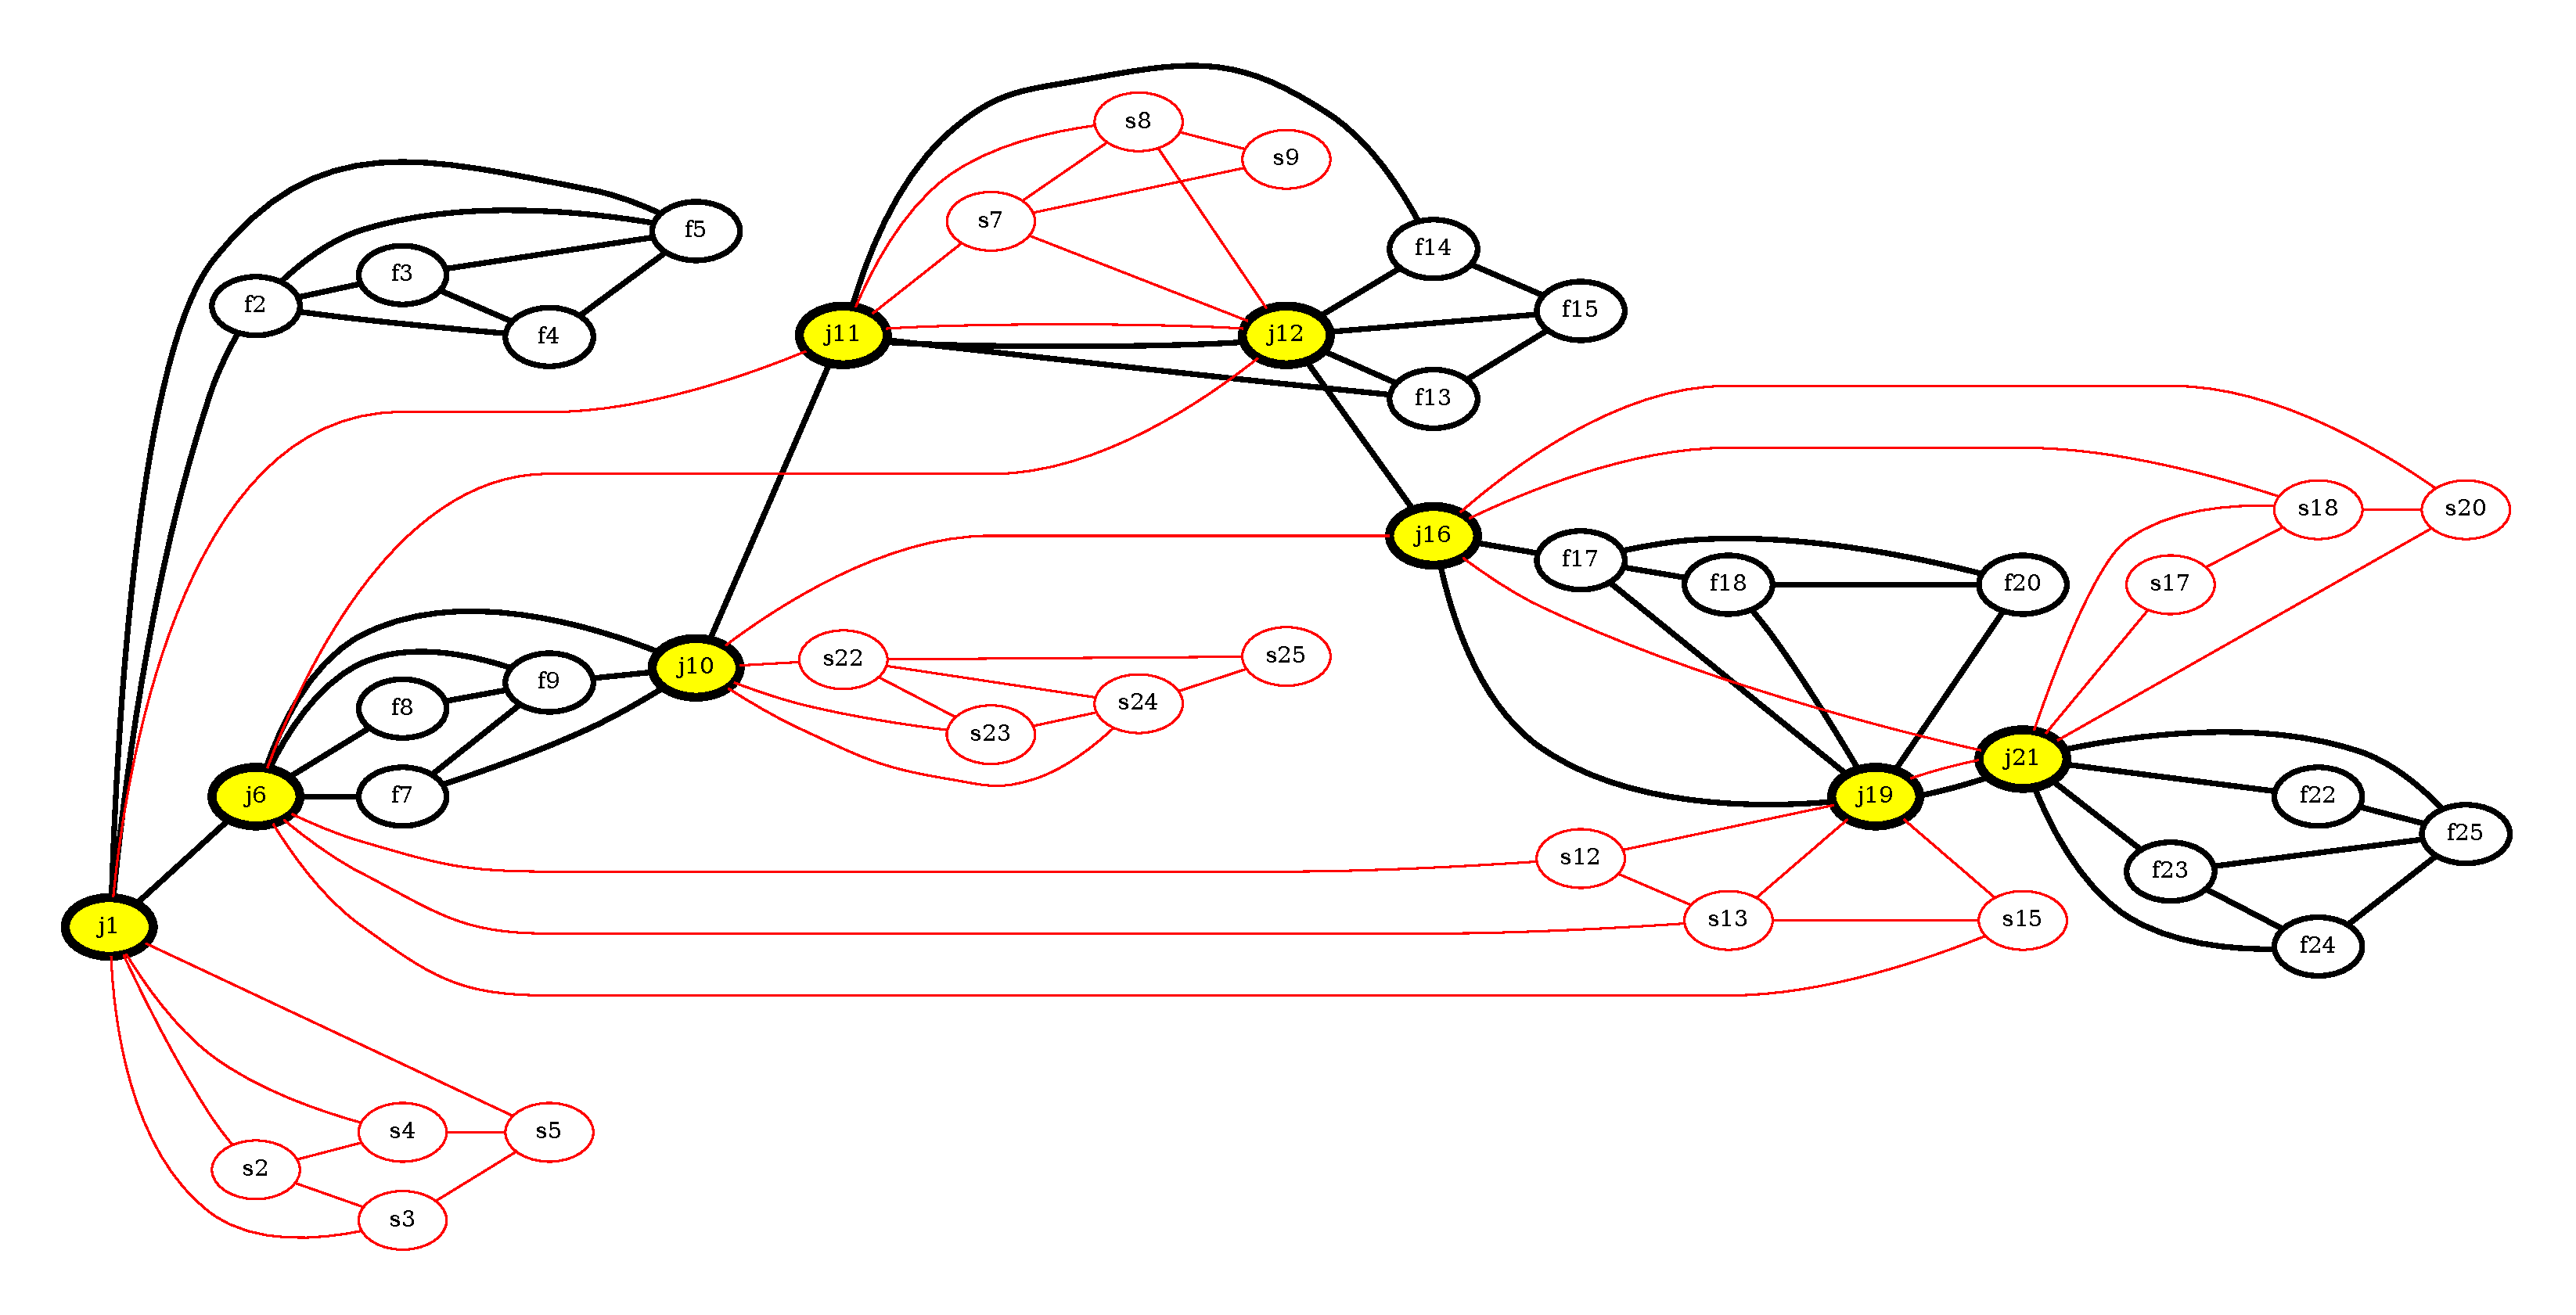
\includegraphics[width=\textwidth]{./sample_jUFLP.pdf}%
    \caption{Sample j-UFLP instance graph.}%
    \label{fig:sample-jUFLP}%
\end{figure}

\section{Solution methods}
\label{sec:org7feacdf}
A naive MIP reformulation for \eqref{eq:j-UFLP} implies introducing new binary
variables \(y_{i,a}^t\) indicating whether point \(i\) in subproblem \(t\) was covered
at least \(a\) times. Therefore, the equivalent problem is:

\begin{subequations}\label{eq:j-UFLP-MIP}
\begin{align}\tag{j-UFLP-MIP}
  \min & \sum_{i=1, t=1,2}^N \Big(c^t_i x^t_i + \sum_{a=0}^{|S_i^t}q_{i,a}^t y^t_{i,a}\Big)+C&\\
    \textrm{s.t. } & \sum_{a=1}^{|S_i|} y_{i,a}^t = \sum_{j\in S^t_i} x^t_i& \textrm{ for all } i=1,\ldots, N, t=1,2,\\
    & y^t_{i,a} \geq y^t_{i, a+1} & \textrm{ for all }i=1, \ldots, N, t=1,2, a=0,\ldots,|S_i|,\\
    & x^t_i\in\{0,1\} & \textrm{ for all } i=1,\ldots,N, t=1,2,\\
    & x^1_i = x^2_j & \textrm{ for all } (i, j)\in J,\label{eq:link}
\end{align}
\end{subequations}
where \(q_{i,a}=f_i^t(a)-f_i^t(a-1)\) and \(C=\sum_{i,t} f_i^t(0)\) are constants.

From the other hand, such problem can be represented as a CPP with two
fixed-width diagrams (each corresponding to a subproblem), having different
order of variables. For each subproblem, we build a BDD, where each path
captures total cost stemming from this subproblem and corresponding to the
respective location decisions. Interconnection between subproblems is achieved
by renaming the variables in the diagrams: for each \((i, j)\in J\) labels of the
BDD layers corresponding to \(x_i^1\) and \(x_j^2\) (in the first and the second
BDD, respectively) must coincide.

\hl{I think this part will go to the appendix:}

Let us briefly illustrate the BDD construction procedure for a single subproblem
with Figure \ref{fig:caves}. Assume we have four clusters of points, denoted \texttt{C1},
\(\ldots\), \texttt{C4} and points \texttt{1}, \(\ldots\), \texttt{6} are endpoints of the edges
connecting these clusters. First, observe that when we fix values for \(x_1\) and
\(x_2\), the costs contribution to the objective stemming from cluster \texttt{C1} can be
obtained by solving a smaller mixed-integer program. The formulation is similar
to \eqref{eq:j-UFLP-MIP}, but with index \(t\) and linking condition \eqref{eq:link}
dropped and the set of nodes restricted to \texttt{C1}. Such MIP would have only \(M\)
variables \(x_i\), corresponding to \texttt{C1}. Therefore, we introduce \(x_1\) and \(x_2\)
to the BDD and capture the costs stemming from cluster \texttt{C1} in BDD arc weights
pointing towards the \(2^2=4\) nodes in the last layer, for \((x_1,x_2)\) being
equal \((0,0)\), \((1,0)\), \((0,1)\), and \((1,1)\), respectively. If we further add
\(x_3\) and \(x_4\) to the diagram, we can fix costs stemming from cluster \texttt{C2} in
BDD arc costs as well. After we add \(x_3\) the diagram width increases to \(2^3=8\)
(we are keeping track of \(x_1\), \(x_2\), and \(x_3\)), but after we introduce \(x_4\)
we do not need to have \(2^4=16\) nodes in the last layer. Note that \(x_1\) will
not affect any costs stemming from \texttt{C3} and \texttt{C4}. Therefore, BDD nodes
corresponding to different values of these two variables in the last layer can
be joined, which would make it sufficient to have \(x_4\) layer with \(4\) nodes
only. Continuing this process, we build a diagram of width \(2^2=8\) at most
(regardless of \(n\) and \(M\)), that encodes the subproblem. Note that depending on
costs, it may or may not be quasi-reduced. The resulting BDD is presented in
Figure \ref{fig:dcloud-DD}. We indicate selected arc costs in the figure, denoting
the objective for the cluster subproblem \texttt{C1} as \(C1(x_1, x_2)\), for \texttt{C2} as
\(C2(x_1, x_2, x_3, x_4)\), for \texttt{C3} as \(C3(x_3, x_4, x_5, x_6)\), and for \texttt{C4} as
\(C4(x_5, x_6)\). Note that because we drop the information regarding specific
choices of \(x_1\) and \(x_2\) the highlighted nodes in Layer 4 will yield only two
child nodes in Layer 5. Note that the natural order of variables that allows
such compact BDD representation is determined by the sequence of clusters in the
figure. Finally, if we have another subproblem encoded by a BDD with variables
\(x_1^\prime, \ldots, x_6^\prime\), and \(J=\{(1,6), (2,5), (3,4), (4,3), (5,2), (6,1)\), we could
reformulate the j-UFLP as a Consistent Path problem instance by renaming the
variables in the diagram depicted in Figure \ref{fig:dcloud-DD} from \((x_1, x_2,
x_3, x_4, x_5, x_6)\) to \((x^\prime_6, x^\prime_5, x^\prime_4, x^\prime_3,
x^\prime_2, x^\prime_1)\).

  \begin{figure}%
    \centering
    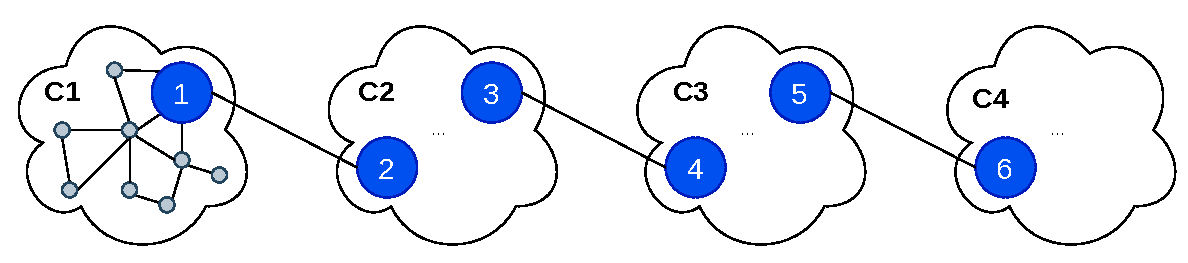
\includegraphics[width=\textwidth]{./caves.pdf}%
    \caption{Sample j-UFLP subproblem graph.}%
    \label{fig:caves}%
\end{figure}


  \begin{figure}%
    \centering
    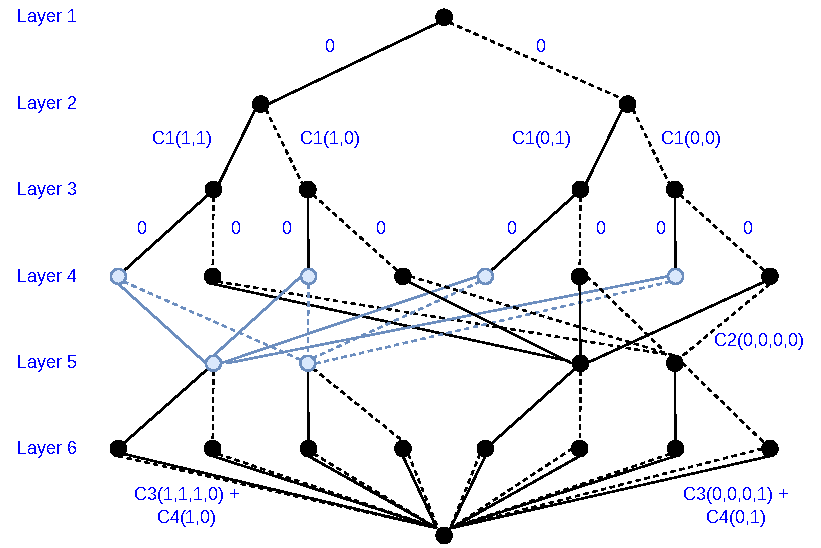
\includegraphics[width=\textwidth]{./dcloud-DD.pdf}%
    \caption{Resulting BDD for the subproblem in Figure \ref{fig:caves}.}%
    \label{fig:dcloud-DD}%
\end{figure}

\section{Numerical performance}
\label{sec:org333aca4}
We generated approximately 400 instances for each value of \(n\) (number of
clusters), ranging from 5 to 14. Each cluster contained \(M=5\) nodes, with
sparsity parameter \(L=0.25\). The latter implies that the number of randomly
generated edges \(|E_k|\) in the cluster satisfies: $$L = 1 - \frac{|E_k|}{M(M-1)
/ 2},$$ assuming one quarter of all possible \(M(M-1)/2\) edges are not present.
We then solved each of the instances with each of the two methods.
\begin{itemize}
\item First, we used a naive MIP formulation \eqref{eq:j-UFLP-MIP} (denoted \texttt{MIP} in
the figures below).
\item Second, we used the pre-defined data regarding the composition of the clusters
to build two BDDs as discussed above. The resulting CPP instance was solved by
aligning the diagrams and finding a shortest path between root and terminal
nodes. The diagrams were aligned using the proposed variable-sequence based
heuristic (denoted \texttt{VS-heuristic}) and a simple baseline of aligning
the second diagram to match the order of the first one (denoted \texttt{to A}).
\end{itemize}

The results are presented in Figure \ref{fig:jUFLP-nums}. On the left panel we
present runtimes for each of the solved instances, one point per instance.
Solution time in seconds (logarithmic scale) is along the vertical axis, number
of clusters \(n\) is along the horizontal axis. We see that since we are
leveraging the additional information regarding the composition of the clusters
in the BDD-based approach, VS-based heuristic tends to perform relatively better
than the naive MIP, and this gap increases as the instance size grows. (Numbers
in the rectangles above the graph indicate the share of instances where the
proposed heuristic were faster at least by 10\%.) On the right panel we present
histograms of the runtimes for \texttt{MIP} and \texttt{to A} heuristics, relative to the
proposed \texttt{VS-heuristic}. The value of 1.0 (vertical line) implies that the
heuristic takes the same time (for a particular instance) as \texttt{VS-heuristic}.
Values to the left of the vertical line imply the heuristic outperforms the
proposed one. We see that while for \(n=7\) clusters \texttt{VS-heuristic} is almost
always slower than MIP, for larger instances it starts to outperform the
baseline on more than two thirds of the instances.

  \begin{figure}%
    \centering
    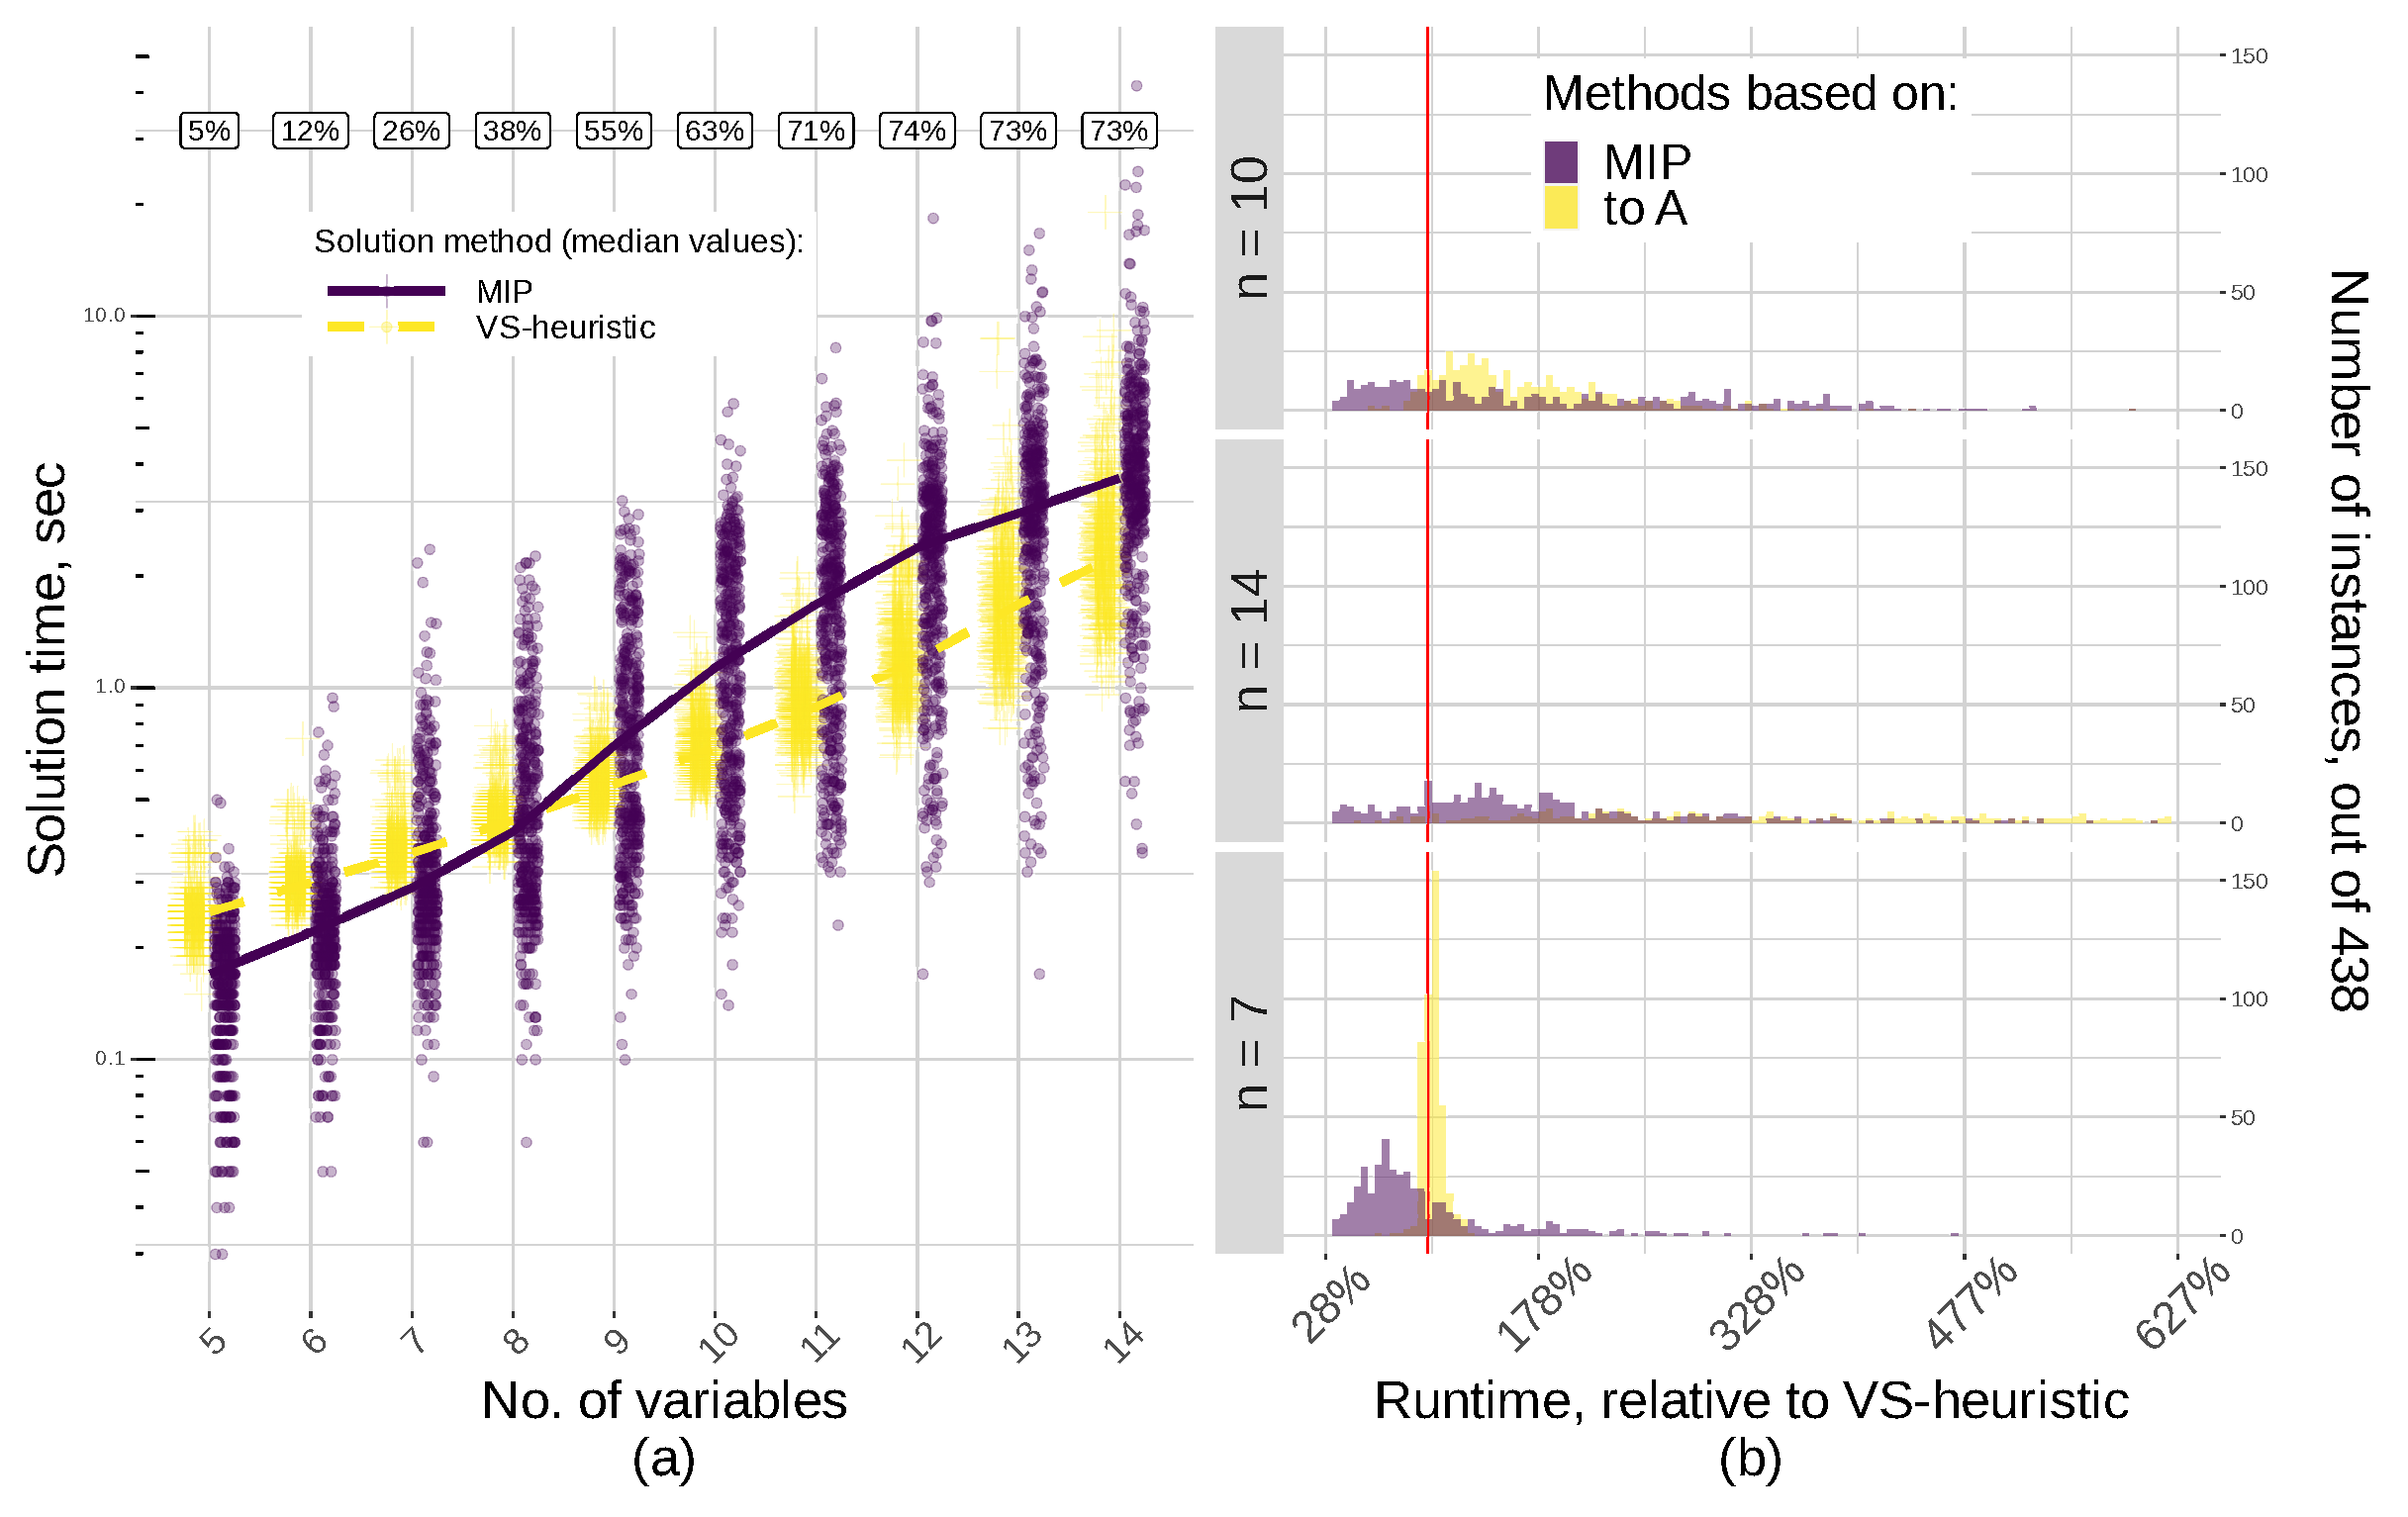
\includegraphics[width=\textwidth]{./jUFLP.eps}%
    \caption{Numerical performance of various heuristics for j-UFLP.}%
    \label{fig:jUFLP-nums}%
\end{figure}

\printbibliography
\end{document}